\documentclass[10pt,a4paper]{article}
\usepackage[a4paper,margin=17mm,headheight=15pt,footskip=13mm]{geometry}
\usepackage{fontspec}
\setmainfont{Noto Sans}
\setsansfont{Inter}
\setmonofont{DejaVu Sans Mono}[Scale=0.84]
\usepackage{amsmath,amssymb,mathtools}
\usepackage{microtype}
\usepackage{xcolor}
\usepackage{booktabs,longtable,tabularx,array,multirow,colortbl}
\usepackage{enumitem}
\usepackage{fancyhdr}
\usepackage{titlesec}
\usepackage{caption}
\usepackage{float}
\usepackage{graphicx}
\usepackage{tcolorbox}
\tcbuselibrary{breakable,skins}
\usepackage{fvextra}
\usepackage{hyperref}
\usepackage{bookmark}
\usepackage{lastpage}
\usepackage{ragged2e}
\usepackage{seqsplit}
\usepackage{pdflscape}

\definecolor{UGTSNavy}{HTML}{0D2B3A}
\definecolor{UGTSTeal}{HTML}{16979B}
\definecolor{UGTSGold}{HTML}{D4A21B}
\definecolor{UGTSCoral}{HTML}{CF6A5A}
\definecolor{UGTSPurple}{HTML}{6B5D96}
\definecolor{UGTSGreen}{HTML}{3F8D6A}
\definecolor{UGTSLight}{HTML}{EDF6F6}
\definecolor{UGTSLightGold}{HTML}{FBF5E4}
\definecolor{UGTSLightPurple}{HTML}{F2EFF8}
\definecolor{UGTSGrey}{HTML}{66737B}
\definecolor{UGTSDark}{HTML}{15252E}
\definecolor{UGTSRedLight}{HTML}{FAECE9}

\hypersetup{
  colorlinks=true,
  linkcolor=UGTSTeal,
  urlcolor=UGTSPurple,
  citecolor=UGTSTeal,
  pdftitle={UGTS-KC 3.6.3 SARA - Seed-Address Referential Algebra},
  pdfauthor={Tom Klootwijk (requester-supplied attribution)},
  pdfsubject={Safe formal integration of BIP39, BIP32, BIP84 and Bech32 into the UGTS referential substrate},
  pdfkeywords={UGTS, BIP39, BIP32, BIP84, Bech32, P2WPKH, cryptography, wallet conformance, authorization, security boundary}
}

\pagestyle{fancy}
\fancyhf{}
\fancyhead[L]{\sffamily\small\color{UGTSNavy}\textbf{UGTS-KC 3.6.3 -- SARA}}
\fancyhead[R]{\sffamily\small\color{UGTSGrey}Seed-Address Referential Algebra}
\fancyfoot[L]{\sffamily\scriptsize\color{UGTSGrey}Tom Klootwijk -- requester-supplied attribution}
\fancyfoot[R]{\sffamily\scriptsize\color{UGTSGrey}Page \thepage\ of \pageref{LastPage}}
\renewcommand{\headrulewidth}{0.4pt}
\renewcommand{\footrulewidth}{0pt}

\titleformat{\section}{\sffamily\Large\bfseries\color{UGTSNavy}}{\thesection}{0.65em}{}
\titleformat{\subsection}{\sffamily\large\bfseries\color{UGTSTeal}}{\thesubsection}{0.55em}{}
\titleformat{\subsubsection}{\sffamily\normalsize\bfseries\color{UGTSPurple}}{\thesubsubsection}{0.5em}{}
\titlespacing*{\section}{0pt}{2.0ex plus .4ex minus .2ex}{0.8ex}
\titlespacing*{\subsection}{0pt}{1.5ex plus .3ex minus .2ex}{0.5ex}

\captionsetup{font=small,labelfont={bf,color=UGTSNavy},textfont={color=UGTSGrey},justification=centering}
\setlist[itemize]{leftmargin=1.5em,itemsep=0.25em,topsep=0.35em}
\setlist[enumerate]{leftmargin=1.7em,itemsep=0.3em,topsep=0.35em}
\setlength{\parindent}{0pt}
\setlength{\parskip}{0.50em}
\emergencystretch=2em

\newtcolorbox{decisionbox}[1][]{enhanced,breakable,colback=UGTSLight,colframe=UGTSTeal,boxrule=0.9pt,arc=1.8mm,left=2.5mm,right=2.5mm,top=1.7mm,bottom=1.7mm,fonttitle=\sffamily\bfseries,title=FORMAL DECISION,#1}
\newtcolorbox{definitionbox}[1][]{enhanced,breakable,colback=UGTSLightPurple,colframe=UGTSPurple,boxrule=0.8pt,arc=1.6mm,left=2.5mm,right=2.5mm,top=1.6mm,bottom=1.6mm,fonttitle=\sffamily\bfseries,title=FORMAL DEFINITION,#1}
\newtcolorbox{proofbox}[1][]{enhanced,breakable,colback=UGTSLightGold,colframe=UGTSGold,boxrule=0.8pt,arc=1.6mm,left=2.5mm,right=2.5mm,top=1.6mm,bottom=1.6mm,fonttitle=\sffamily\bfseries,title=DERIVATION / INVARIANT,#1}
\newtcolorbox{boundbox}[1][]{enhanced,breakable,colback=UGTSRedLight,colframe=UGTSCoral,boxrule=0.8pt,arc=1.6mm,left=2.5mm,right=2.5mm,top=1.6mm,bottom=1.6mm,fonttitle=\sffamily\bfseries,title=SECURITY / EVIDENCE BOUNDARY,#1}
\newtcolorbox{metricbox}[1][]{enhanced,breakable,colback=white,colframe=UGTSGreen,boxrule=0.8pt,arc=1.6mm,left=2.5mm,right=2.5mm,top=1.6mm,bottom=1.6mm,fonttitle=\sffamily\bfseries,title=EXACT METRICS,#1}

\newcommand{\code}[1]{\texttt{#1}}
\newcommand{\Ftwo}{\mathbb F_2}
\newcommand{\N}{\mathbb N}
\newcommand{\sha}{\operatorname{SHA256}}
\newcommand{\hmac}{\operatorname{HMAC\!\mbox{-}SHA512}}
\newcommand{\HashOneSixty}{\operatorname{RIPEMD160}\!\circ\!\operatorname{SHA256}}

\begin{document}
\pagenumbering{gobble}

\begin{titlepage}
\pagecolor{UGTSNavy}
\color{white}
\vspace*{8mm}
{\sffamily\bfseries\fontsize{34}{39}\selectfont UGTS-KC 3.6.3 -- SARA\par}
\vspace{4mm}
{\sffamily\fontsize{21}{25}\selectfont Seed-Address Referential Algebra\par}
\vspace{6mm}
{\sffamily\large Public deterministic-wallet standards packed into the referential substrate\par}
\vspace{11mm}

\begin{tcolorbox}[enhanced,colback=white,colframe=UGTSTeal,boxrule=1.2pt,arc=2mm,left=5mm,right=5mm,top=4mm,bottom=4mm]
\color{UGTSDark}
\textbf{Integrated mechanisms}\par
BIP39 entropy, checksum and 11-bit word cells; an ordered mnemonic cell complex; NFKD and the standard seed transition; a typed BIP32 derivation tree with distinct normal and hardened edges; the BIP84 P2WPKH route; compressed public-key and HASH160 projection; witness-program/script relations; Bech32 and Bech32m validation; public-only certificates; an explicit authorization guard; non-enumerating search-space metrics; and a canonical handoff to the UGTS event calculus.
\end{tcolorbox}

\vspace{6mm}
\begin{tcolorbox}[enhanced,colback=UGTSRedLight,colframe=UGTSCoral,boxrule=1.1pt,arc=2mm,left=5mm,right=5mm,top=3.5mm,bottom=3.5mm]
\color{UGTSDark}
\textbf{Non-negotiable boundary}\par
This version does not implement or document a real-wallet brute-force engine. It contains no mnemonic/passphrase enumeration, private-key scan, target-address preimage loop, signing, transaction broadcast, balance targeting or funds-transfer path. The supplied address is used only as a public checksum, witness-program and script fixture.
\end{tcolorbox}

\vfill
{\sffamily\Large\bfseries Tom Klootwijk\par}
{\sffamily\large Principal Creative Technologist\par}
{\sffamily\large 10-07-1990 \quad NL200678942\par}
\vspace{3mm}
{\sffamily\small Name, title, date and identifier are requester-supplied and were not independently verified.\par}
\vspace{9mm}
{\sffamily\small Version 3.6.3 -- 18 August 2026\par}
{\sffamily\small Standards-derived cryptographic operators are separated from engineering-derived UGTS integration and rejected attack scopes.\par}
\end{titlepage}
\nopagecolor
\color{UGTSDark}

\section*{Abstract}
Version 3.6.3 extends the 3.6.2 packed geometric-topological substrate with a cryptographic representation profile. The new profile does not turn a wallet into geometry and does not claim that topology weakens cryptography. It uses the same referential discipline: every object has a type, every transform has a domain and codomain, every packed record has a schema, every guard has an explicit reason code, and every public result has lineage.

The standards path is represented as
\[
\begin{aligned}
\text{entropy}&\to\text{checksum}\to\text{11-bit word cells}\to\text{mnemonic}\\
&\to\text{transient seed}\to\text{HD tree}\to\text{public key}\\
&\to\text{witness program}\to\text{address}.
\end{aligned}
\]
The implementation validates official public test vectors, decodes public addresses, produces public-only certificates, validates self-owned known inputs, and calculates optimistic feasibility metrics without generating candidates. It contains 45 new atomic operators, 19 content-addressed definitions, 20 claims-ledger entries, 42 new tests and all 153 retained tests from earlier versions, for 195 passing tests in total.

\begin{decisionbox}
The requested ``brute-force pentesting'' concept is admitted only as a bounded, non-operational feasibility analysis and authorization gate. A real third-party mainnet key search is rejected. The safe technical core is standards conformance, public decoding, self-owned deterministic reconstruction, watch-only consistency, test-network experimentation and search-space measurement.
\end{decisionbox}

\tableofcontents
\clearpage
\pagenumbering{arabic}

\section{Version lineage, source classes and scope}

\subsection{Inherited substrate discipline}
UGTS-KC 3.6.2 made the authoritative object a packed, typed relation substrate rather than a renderer. SARA preserves that architecture. Cryptographic objects are not collapsed into one bit or one address: entropy, word indices, mnemonic text, seed, chain code, private scalar, public key, script, address, authorization and lineage are distinct types.

The update uses three visibly separate evidence classes:
\begin{center}
\begin{tabularx}{0.96\textwidth}{p{0.20\textwidth}X X}
\toprule
\textbf{Class} & \textbf{Contains} & \textbf{Examples}\\
\midrule
Standards-derived & Transformations explicitly specified by Bitcoin Improvement Proposals. & BIP39 checksum and seed transition; BIP32 child derivation; BIP84 path; BIP141 witness program; BIP173/BIP350 checksums.\\
Engineering-derived & Typed integration that preserves the standards while adding bounds, references and reason codes. & Word-cell complex, authorization guard, public-only certificate, UGTS handoff, schema and content-addressed definitions.\\
Rejected/unsupported & Capabilities that are not needed for conformance and would cross the authorization boundary. & Third-party secret search, passphrase spraying, private-key scanning, signing, broadcasting, balance targeting and funds transfer.\\
\bottomrule
\end{tabularx}
\end{center}

\subsection{Security decision}
Public visibility of an address does not grant permission to recover or use its spending key. The package therefore treats
\begin{Verbatim}[breaklines=true,fontsize=\small]
bc1q7ydrtdn8z62xhslqyqtyt38mm4e2c4h3mxjkug
\end{Verbatim}
as a public syntax fixture only. The requester-provided ownership/context label is recorded as unverified external metadata and never used as legal or cryptographic proof.

\begin{figure}[H]
\centering
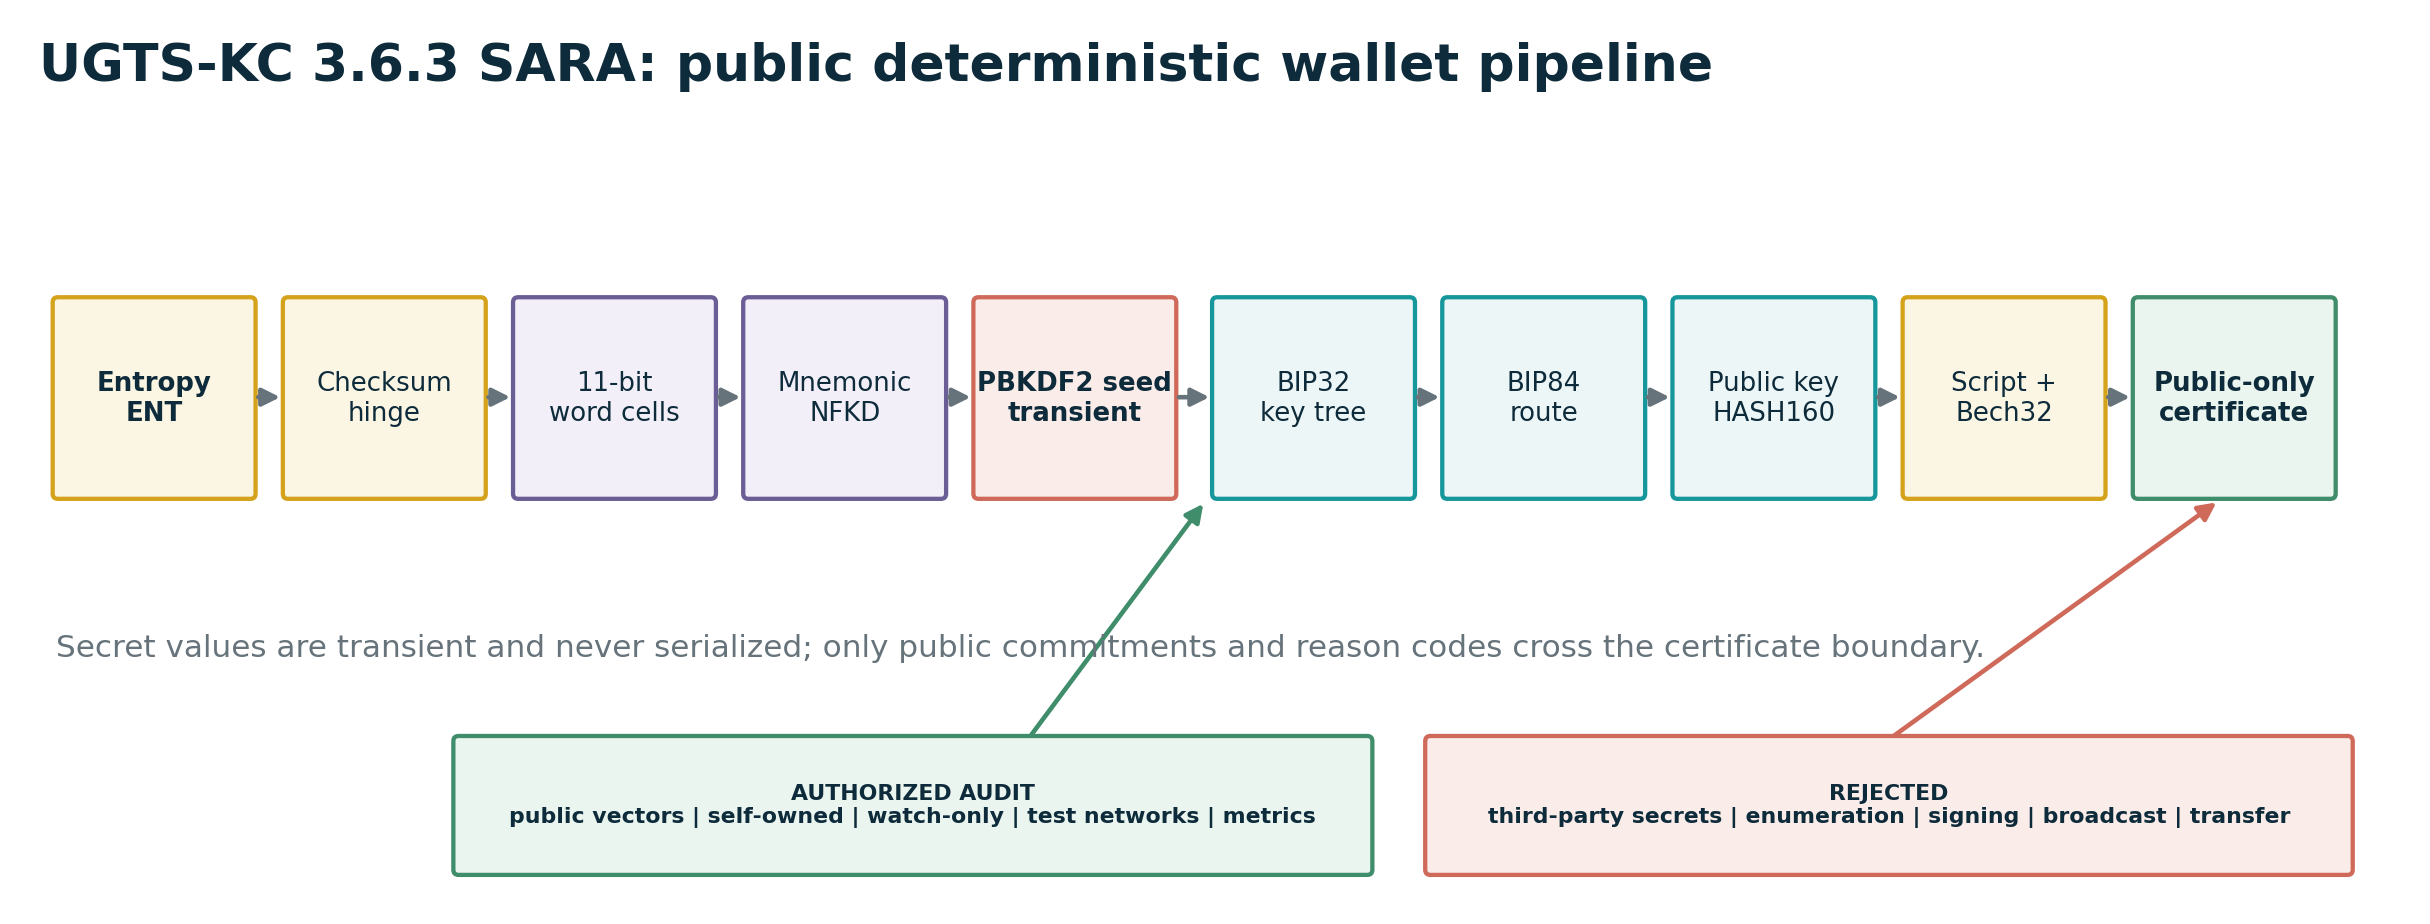
\includegraphics[width=\textwidth]{figures/sara363_architecture.png}
\caption{SARA maps the public standards pipeline into a certificate while keeping secret material transient and attack capabilities outside the profile.}
\end{figure}

\section{Referential cryptographic state}

\subsection{Typed state tuple}
The abstract state is
\[
q_{\mathrm{SARA}}=(P,E,C,W,M,S,N,D,K,H,Q,A,Z,\mathcal A,\mathcal L,U),
\]
where:
\begin{itemize}
\item $P$ is the selected standards/profile identifier;
\item $E$ is entropy and $C$ its checksum prefix;
\item $W$ is the ordered 11-bit word-cell sequence and $M$ the normalized mnemonic;
\item $S$ is the transient 64-byte seed and $N$ a transient HD node;
\item $D$ is the derivation path;
\item $K$ is a compressed public key and $H=\HashOneSixty(K)$;
\item $Q$ is the witness program/script relation and $A$ the human-readable address;
\item $Z$ is a public certificate;
\item $\mathcal A$ is authorization state, $\mathcal L$ lineage and $U$ uncertainty/status.
\end{itemize}

\subsection{Secret/public partition}
\begin{definitionbox}
Let $\mathcal S$ be the secret class and $\mathcal P$ the public class:
\[
\mathcal S=\{E,M,\text{passphrase},S,k,c,\text{xprv},\text{WIF}\},
\]
\[
\mathcal P=\{\text{profile},D,K,H,Q,A,\text{reason codes},\text{public test vectors}\}.
\]
A production certificate is valid only if its serialized field set is disjoint from $\mathcal S$. The reference package additionally has no network client and no transaction capability.
\end{definitionbox}

The sample certificate uses a universally published test mnemonic, but it still omits mnemonic- and seed-derived fingerprints. The retained four-byte BIP32 parent fingerprint is only a routing hint and is not treated as a collision-free identity.

\subsection{Referential definitions}
Each definition record contains a stable ID, type, domain, codomain, evaluation phase, dependencies, parameters, invariants, provenance and canonical SHA-256 content hash. References are resolved before evaluation; missing references, duplicate IDs, dependency cycles and hash mismatches are validation failures.

\section{BIP39 as an ordered word-cell complex}

\subsection{Entropy, checksum and cells}
For $\mathrm{ENT}\in\{128,160,192,224,256\}$,
\[
\mathrm{CS}=\frac{\mathrm{ENT}}{32},\qquad
\mathrm{MS}=\frac{\mathrm{ENT}+\mathrm{CS}}{11}.
\]
For entropy bit string $e$, define
\[
b=e\,\Vert\,\operatorname{prefix}_{\mathrm{CS}}(\sha(e)).
\]
The bit string $b$ is partitioned into ordered cells
\[
w_i=b[11i:11(i+1)]\in\{0,\dots,2047\},
\]
and each $w_i$ indexes the committed 2048-word list.

\begin{figure}[H]
\centering
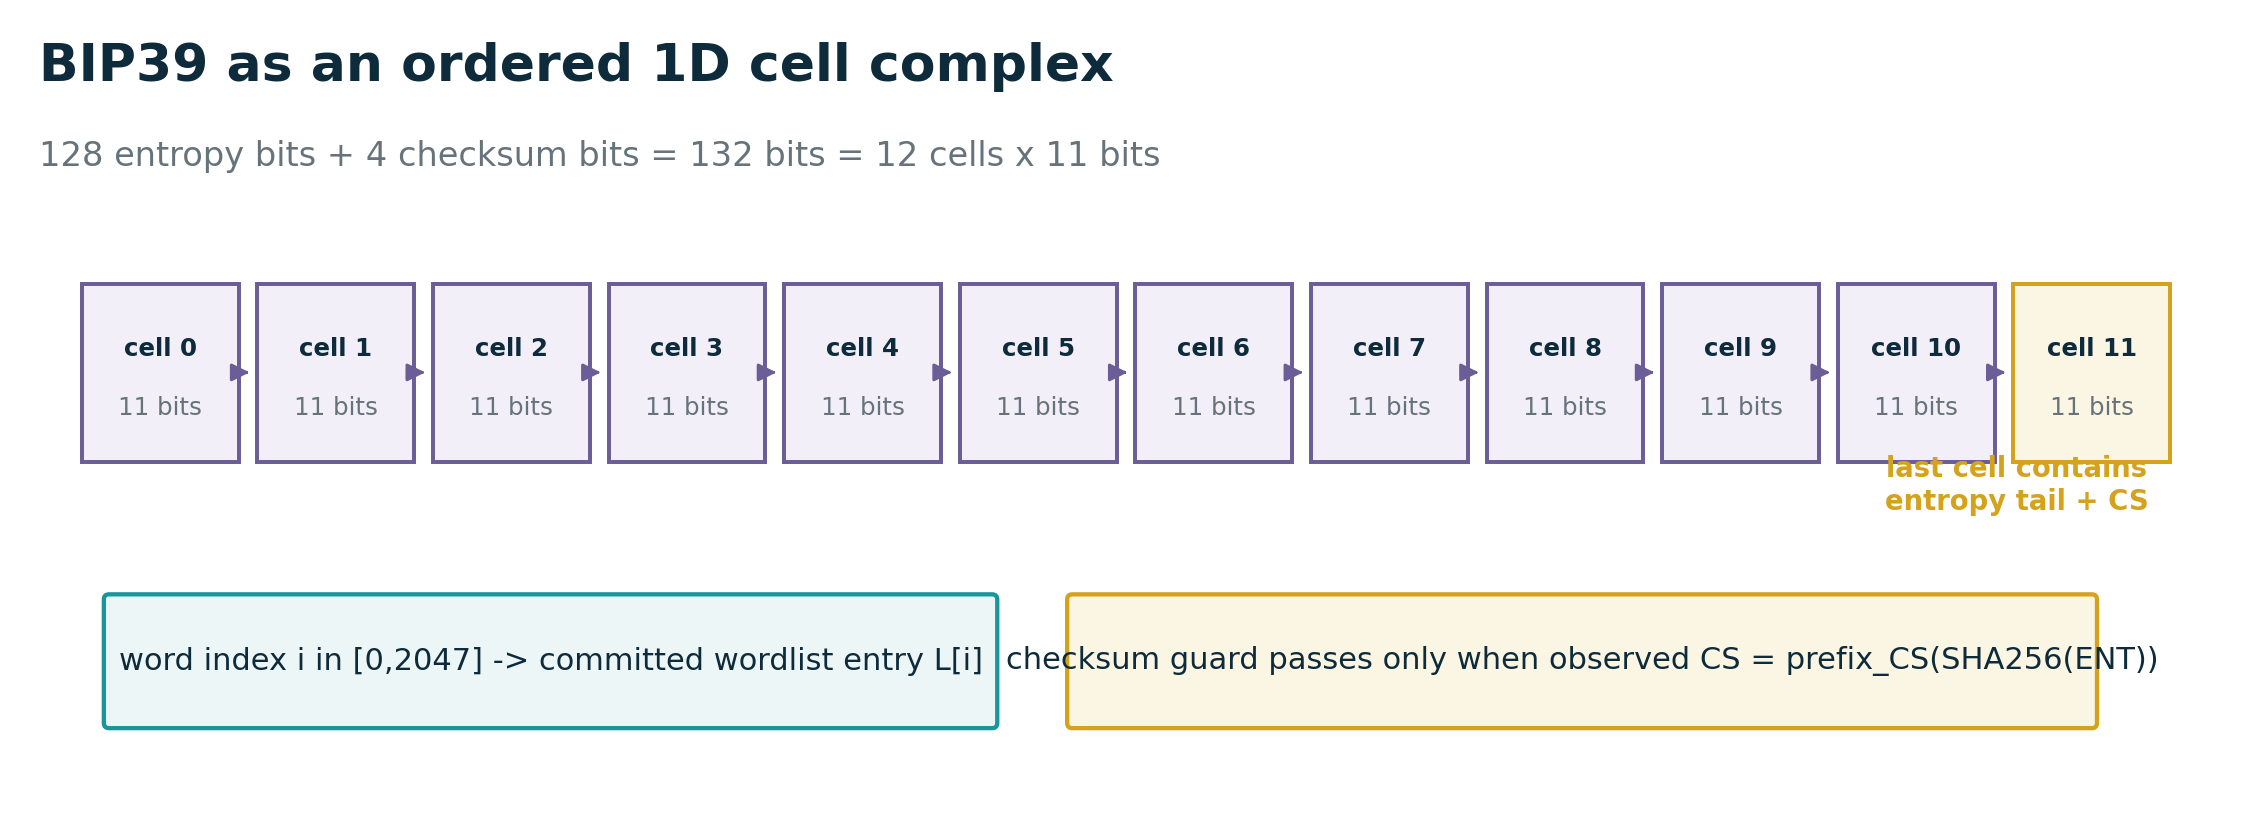
\includegraphics[width=0.97\textwidth]{figures/sara363_word_cells.png}
\caption{A 12-word mnemonic is represented as a path of twelve labeled 11-bit cells; the final cell contains both entropy and checksum bits.}
\end{figure}

\subsection{Cell-complex definition}
Let
\[
X_M=(V,E,\lambda),\quad V=\{v_0,\ldots,v_m\},\quad E=\{(v_i,v_{i+1})\}_{i=0}^{m-1},
\]
with label map $\lambda(v_i)=w_i$. This is a one-dimensional path complex. Its topology records order and adjacency; it does not add cryptographic strength. The wordlist commitment fixes the meaning of every label by count, uniqueness, order, normalization and digest:
\begin{Verbatim}[breaklines=true,fontsize=\small]
BIP39 English list SHA-256:
2f5eed53a4727b4bf8880d8f3f199efc90e58503646d9ff8eff3a2ed3b24dbda
\end{Verbatim}

\subsection{Checksum hinge}
For a candidate cell path, split the recovered bit string into entropy $e'$ and observed checksum $c'$. The checksum guard is
\[
g_{39}(M)=\begin{cases}
0,&c'=\operatorname{prefix}_{\mathrm{CS}}(\sha(e')),\\
1,&\text{otherwise}.
\end{cases}
\]
The path is syntactically admitted only when $g_{39}=0$.

\begin{boundbox}
The checksum is an integrity rule, not an ownership test, password test or balance test. A BIP39 mnemonic transports computer-generated entropy; arbitrary memorable sentences are outside this profile. For 12 words, one in sixteen arbitrary 12-index sequences passes the checksum, but the valid space still contains $2^{128}$ mnemonics.
\end{boundbox}

\subsection{Public test vector}
The package includes the official public 12-word vector
\begin{Verbatim}[breaklines=true,fontsize=\small]
abandon abandon abandon abandon abandon abandon
abandon abandon abandon abandon abandon about
\end{Verbatim}
with indices $(0,0,0,0,0,0,0,0,0,0,0,3)$ and checksum bits $0011$. It is a public conformance vector and must never be used to hold funds.

\section{Seed transition and transient-secret boundary}

After Unicode NFKD normalization, BIP39 defines
\[
S=\operatorname{PBKDF2}_{\hmac}
\left(
\operatorname{NFKD}(M),
\operatorname{NFKD}(\texttt{mnemonic}\Vert p),
2048,64
\right),
\]
where $p$ is the optional passphrase. The output $S$ is a 64-byte seed.

\begin{definitionbox}
The seed transition is an in-memory edge, not a persistent substrate node. The implementation may hold $M$, $p$, $S$, a private scalar and chain code long enough to derive a public test result, but none may cross the certificate serialization boundary. The runtime returns public commitments, path metadata, reason codes and lineage only.
\end{definitionbox}

Every passphrase produces a seed; therefore the standard does not provide an intrinsic ``wrong passphrase'' signal. SARA does not implement passphrase guessing or candidate testing. Self-owned recovery belongs in dedicated audited custody software, not in this reference profile.

\section{BIP32 derivation as a typed tree topology}

\subsection{Extended nodes}
A private extended node is
\[
n=(k,c,d,f,i),
\]
with private scalar $k$, chain code $c$, depth $d$, parent fingerprint $f$ and child number $i$. The master node is obtained by
\[
I=\hmac_{\texttt{Bitcoin seed}}(S),\qquad k=\operatorname{parse}_{256}(I_L),\qquad c=I_R.
\]

For child index $i$, the data term is
\[
\operatorname{data}(i)=
\begin{cases}
\texttt{0x00}\Vert\operatorname{ser}_{256}(k)\Vert\operatorname{ser}_{32}(i),&i\ge2^{31},\\
\operatorname{ser}_P(K)\Vert\operatorname{ser}_{32}(i),&i<2^{31},
\end{cases}
\]
followed by
\[
I=\hmac_c(\operatorname{data}(i)),\qquad
k_i=(\operatorname{parse}_{256}(I_L)+k)\bmod n,\qquad c_i=I_R.
\]
Invalid zero/out-of-range results are rejected according to the standard.

\subsection{Normal and hardened edges}
\begin{figure}[H]
\centering
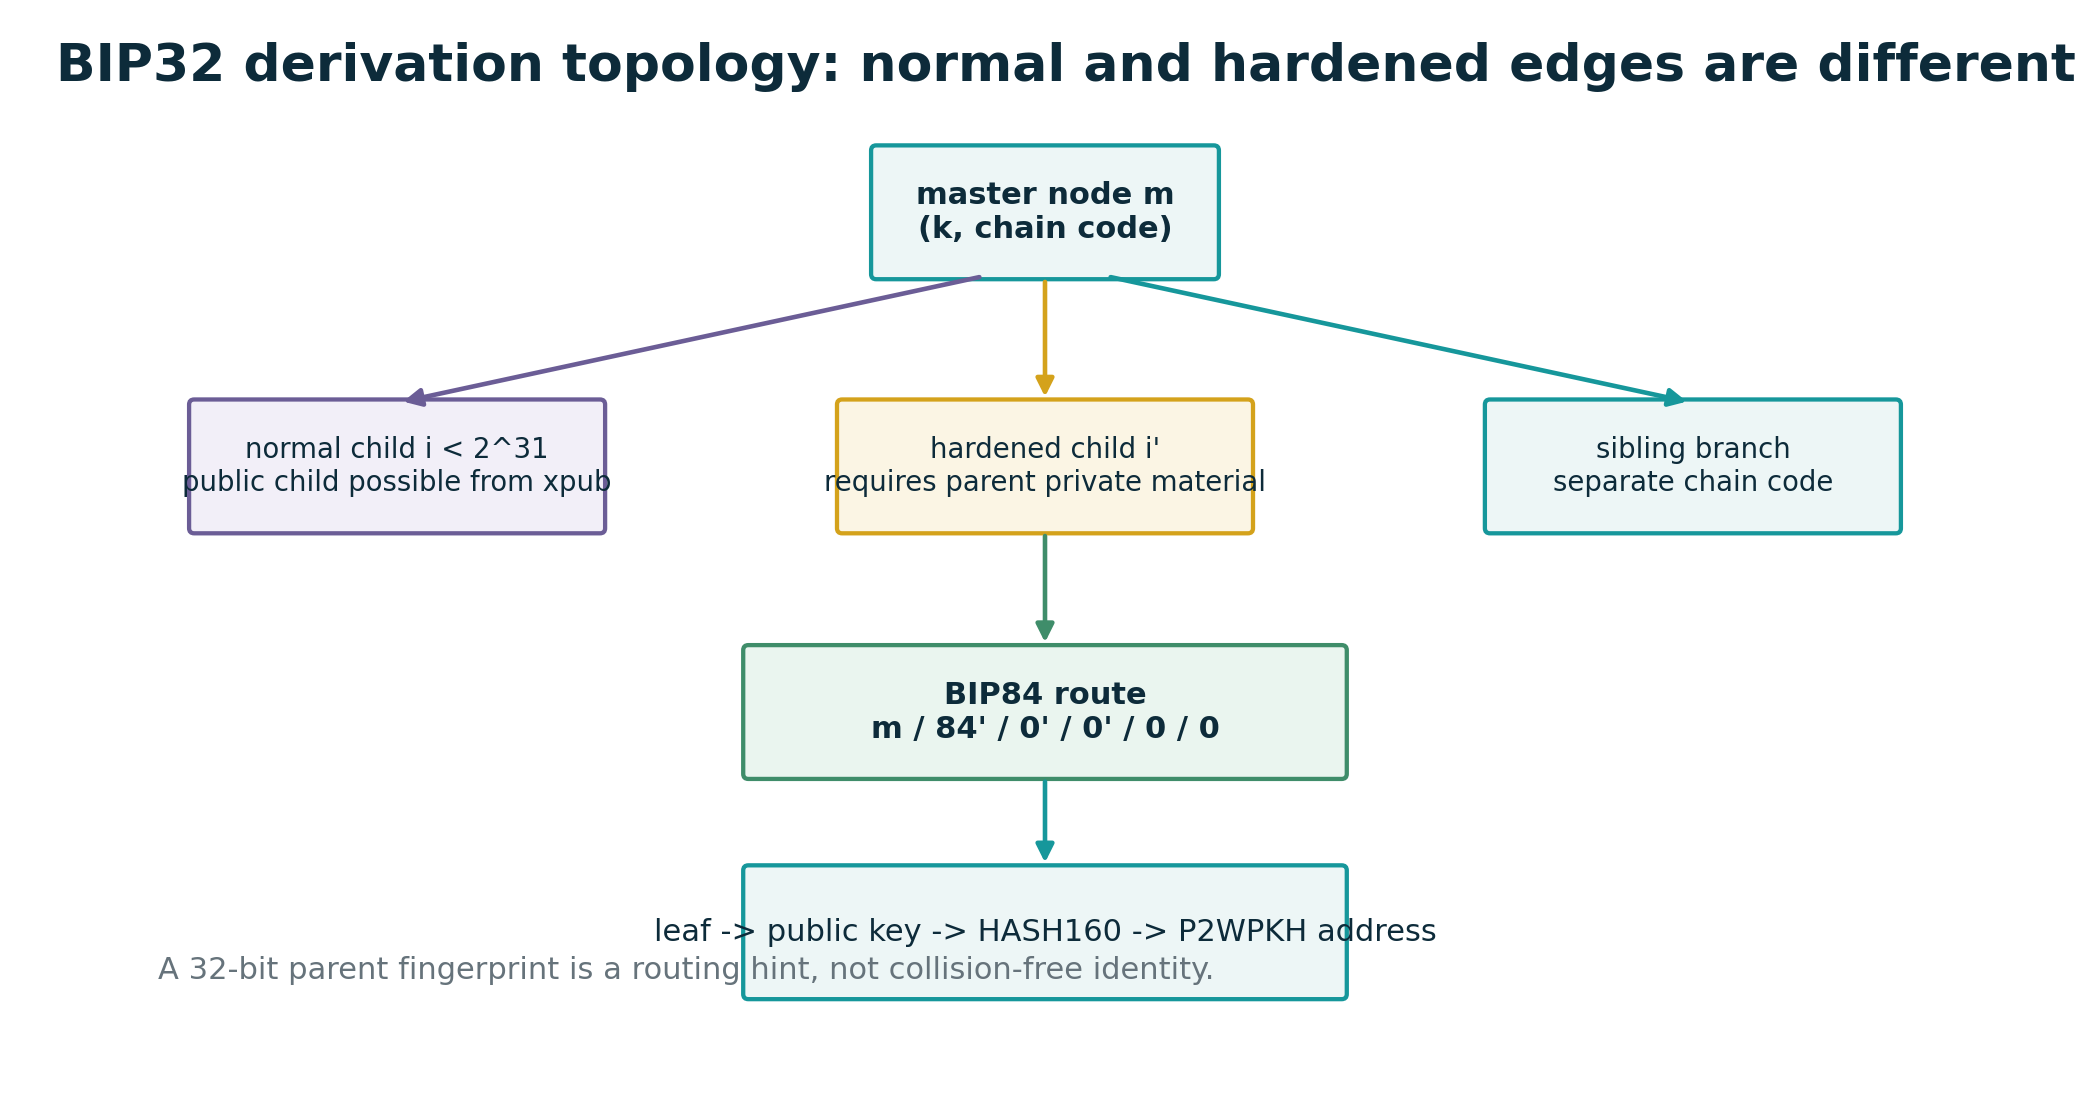
\includegraphics[width=0.82\textwidth]{figures/sara363_hd_tree.png}
\caption{Normal and hardened edges have different derivability and privacy properties; the parent fingerprint is a routing hint, not a collision-free identity.}
\end{figure}

Normal children use indices $0\le i<2^{31}$ and may be derived from an extended public parent. Hardened children use $i\ge2^{31}$ and require private parent material. The edge type is therefore part of the topology, not a formatting detail.

\subsection{BIP44/BIP84 route word}
SARA interprets a path as an ordered edge word. The standard native-SegWit route is
\[
D=\texttt{m/84'/0'/account'/change/index}.
\]
The reference receiving leaf is
\[
\texttt{m/84'/0'/0'/0/0}.
\]
The first three edges are hardened; change and address-index edges are normal. This route is a deterministic namespace, not evidence of ownership.

\section{Public-key, script and address projection}

\subsection{P2WPKH relation}
For private scalar $k$, let $K=\operatorname{ser}_P(kG)$ be the compressed public key and
\[
h=\HashOneSixty(K).
\]
A witness-v0 20-byte program has scriptPubKey
\[
Q=\texttt{0x00}\;\texttt{0x14}\;\Vert\;h.
\]
The mainnet human-readable address is the Bech32 encoding of HRP \code{bc}, witness version 0 and program $h$.

\subsection{Checksum family guard}
For witness version 0, SARA requires Bech32. For witness versions 1--16, it requires Bech32m. The decoder rejects mixed case, invalid characters, checksum failure, invalid witness versions and invalid program lengths. A valid checksum detects many transcription errors; it does not authenticate a person or prove spending authority.

\begin{figure}[H]
\centering
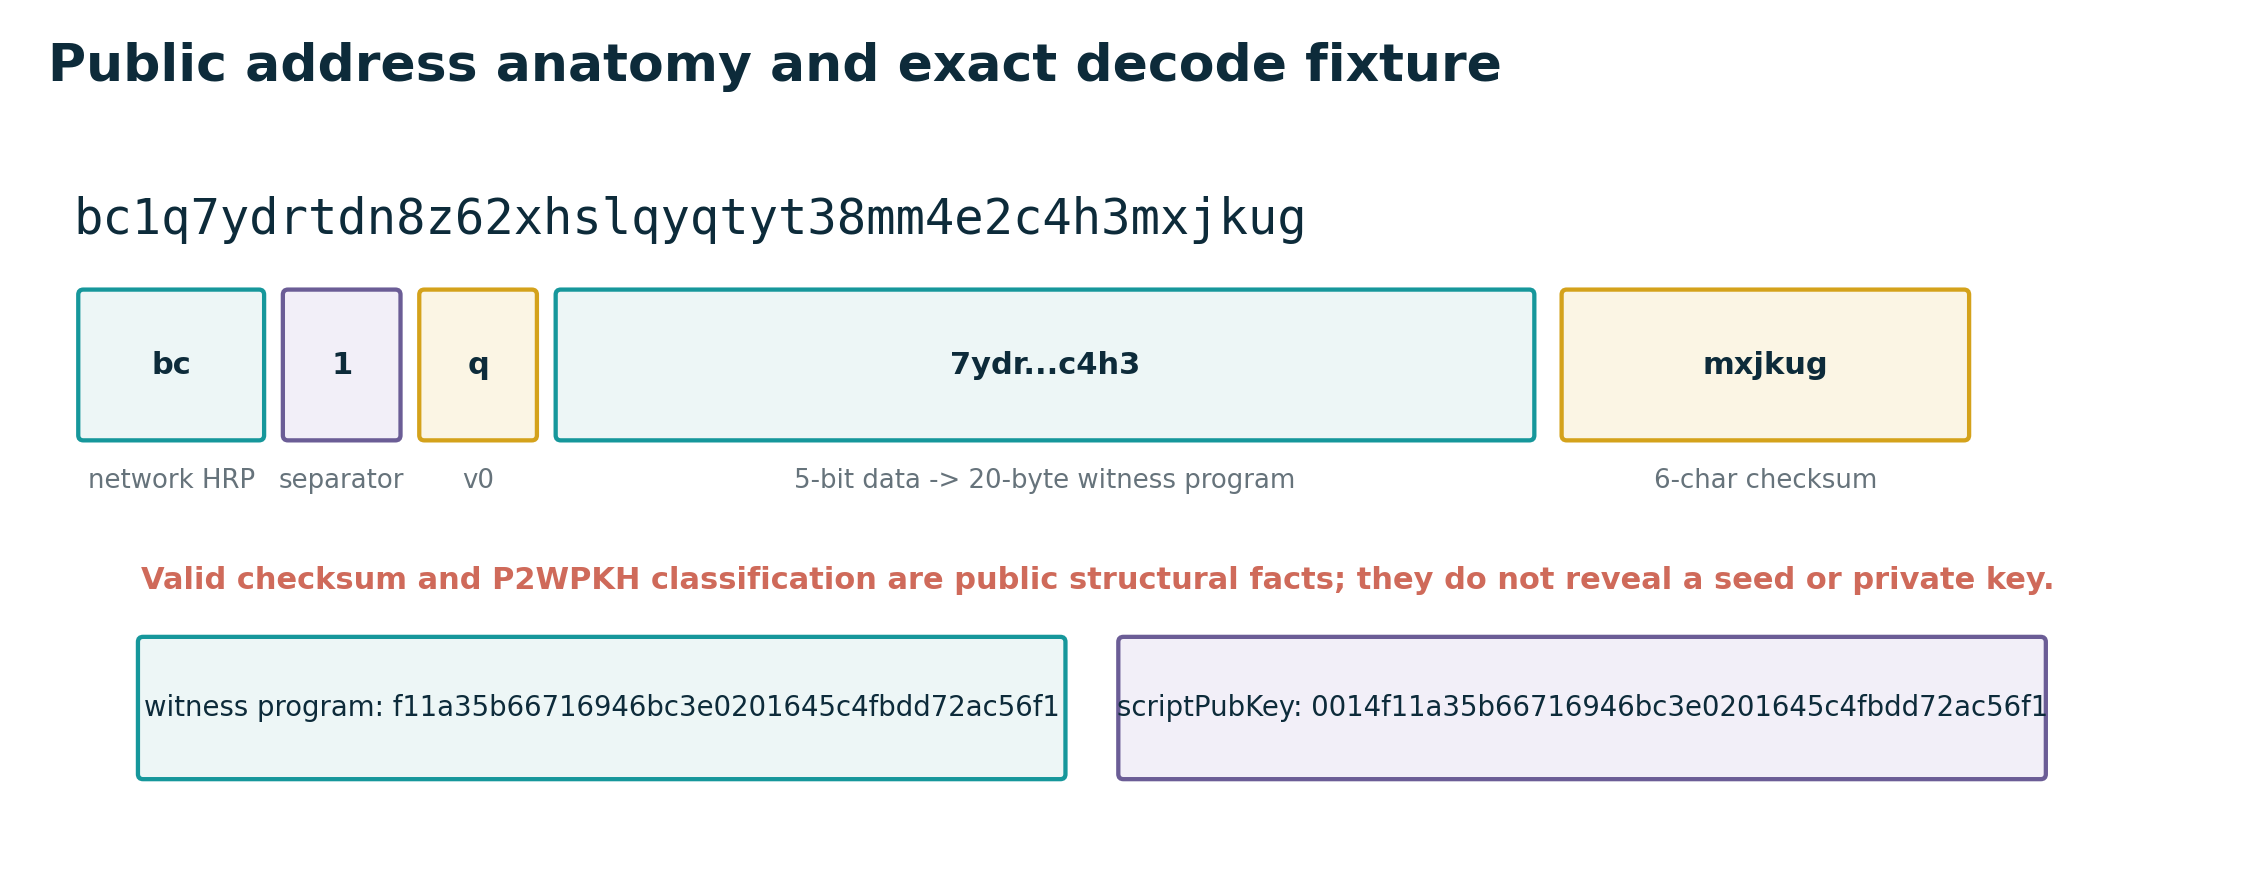
\includegraphics[width=0.95\textwidth]{figures/sara363_address_anatomy.png}
\caption{The supplied address is decomposed into public structural fields. No private or signing material is present.}
\end{figure}

\section{Exact public fixtures}

\subsection{Official BIP84 conformance vector}
The public reference path produces:
\begin{Verbatim}[breaklines=true,fontsize=\small]
path:       m/84'/0'/0'/0/0
pubkey:     0330d54fd0dd420a6e5f8d3624f5f3482cae350f79d5f0753bf5beef9c2d91af3c
HASH160:    c0cebcd6c3d3ca8c75dc5ec62ebe55330ef910e2
script:     0014c0cebcd6c3d3ca8c75dc5ec62ebe55330ef910e2
address:    bc1qcr8te4kr609gcawutmrza0j4xv80jy8z306fyu
\end{Verbatim}
The certificate contains no mnemonic, passphrase, seed, private scalar, chain code, xprv or WIF field.

\subsection{Requester-supplied public address}
The decoder returns:
\begin{center}
\begin{tabularx}{0.96\textwidth}{p{0.27\textwidth}X}
\toprule
\textbf{Field} & \textbf{Exact value}\\
\midrule
Address & \ttfamily\seqsplit{bc1q7ydrtdn8z62xhslqyqtyt38mm4e2c4h3mxjkug}\\
HRP & \code{bc}\\
Checksum family & Bech32; checksum valid\\
Witness version & 0\\
Witness program & \ttfamily\seqsplit{f11a35b66716946bc3e0201645c4fbdd72ac56f1}\\
Program length & 20 bytes\\
Address type & P2WPKH\\
scriptPubKey & \ttfamily\seqsplit{0014f11a35b66716946bc3e0201645c4fbdd72ac56f1}\\
Allowed use & Public format/checksum/witness-program/script decode only\\
\bottomrule
\end{tabularx}
\end{center}

\begin{boundbox}
These fields establish only that the string is structurally a valid mainnet witness-v0 20-byte address. The package does not establish who controls it, whether it currently holds funds, whether a third-party label is accurate, or whether any testing is authorized by an owner or court.
\end{boundbox}

\section{Authorized defensive audit kernel}

\subsection{Authorization predicate}
Let $s$ be a requested scope set. The authorization guard is
\[
\mathcal A(s)=1
\iff
s\subseteq\mathcal S_{\mathrm{allowed}}
\land s\cap\mathcal S_{\mathrm{forbidden}}=\varnothing.
\]
Allowed scopes include public BIP vectors, public address decode, watch-only consistency, checksum validation, self-owned known-seed derivation, regtest/signet/testnet experiments and non-enumerating metrics. Forbidden scopes include third-party mainnet key search, mnemonic permutations, passphrase spraying, private-key scans, target-address preimage search, signing, broadcast and funds transfer.

\begin{figure}[H]
\centering
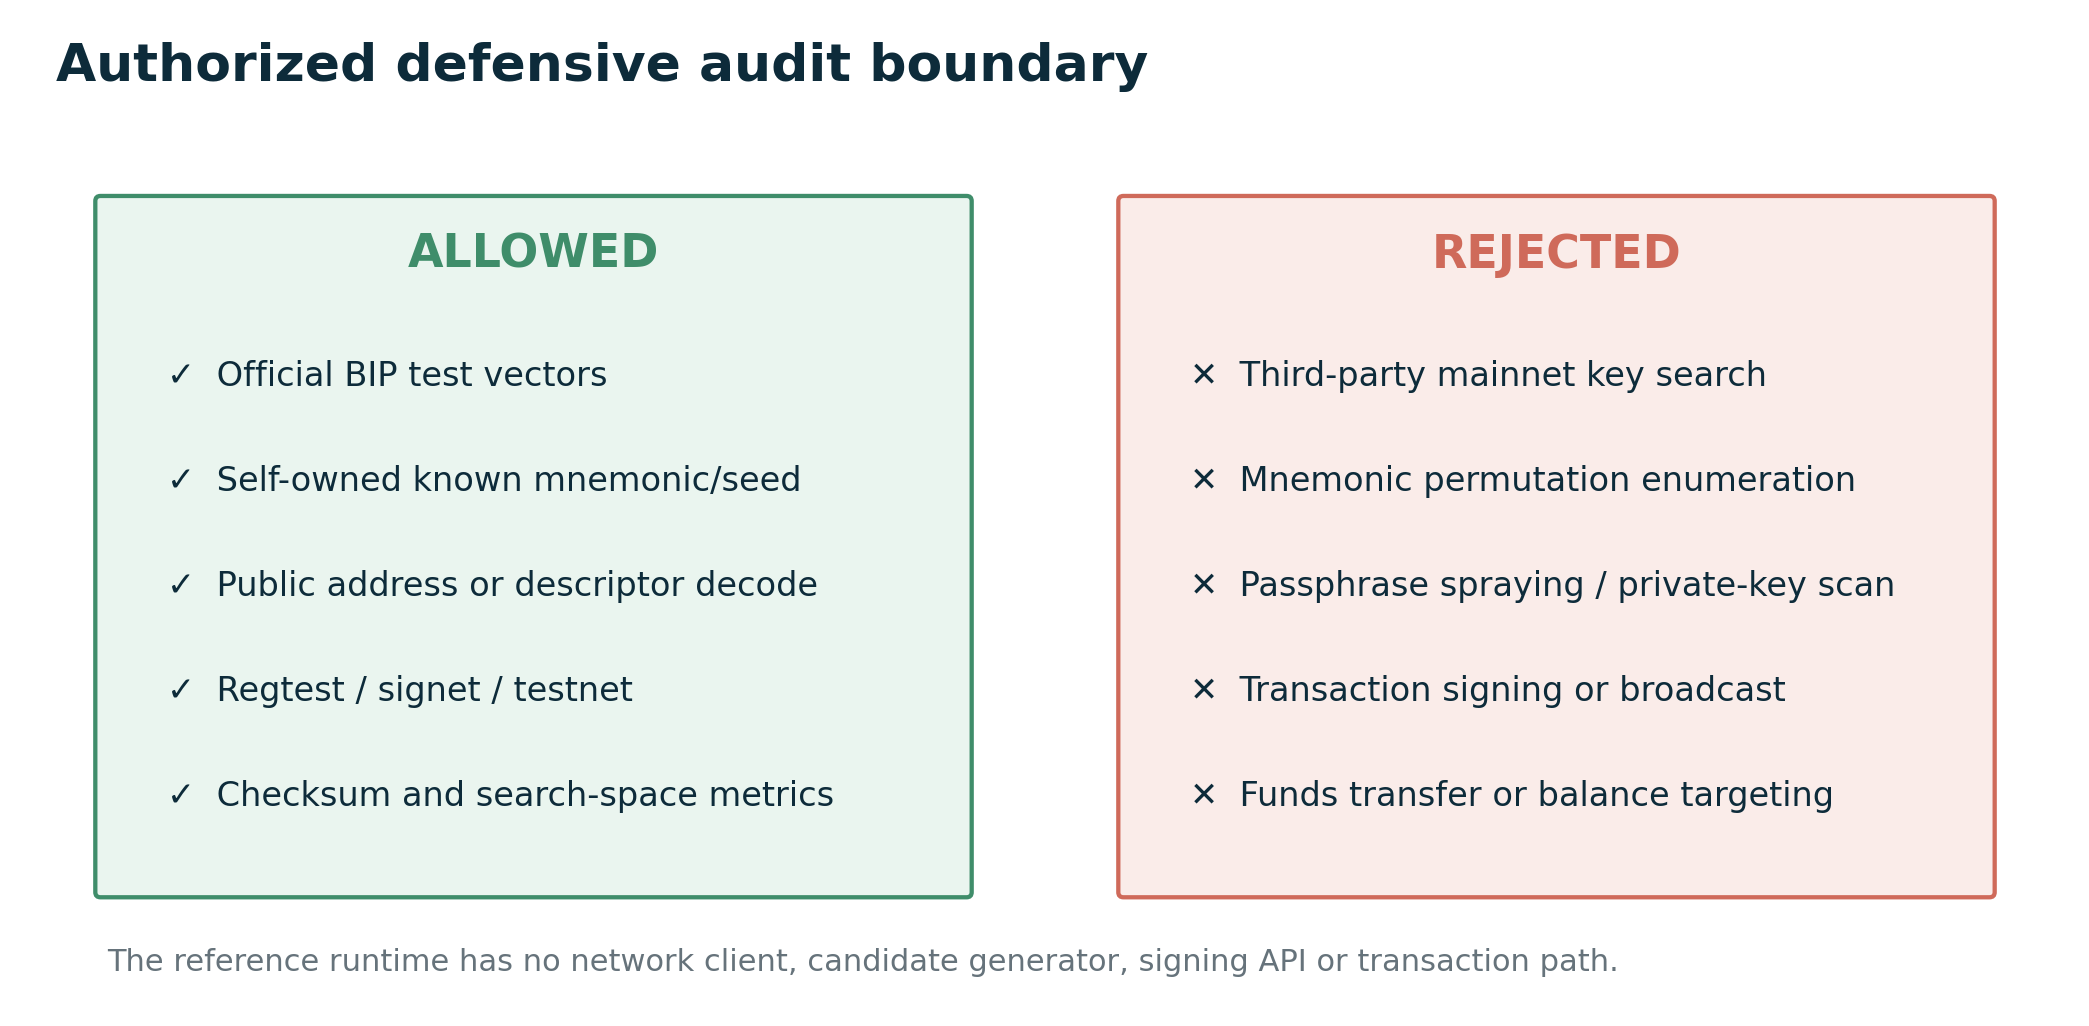
\includegraphics[width=0.86\textwidth]{figures/sara363_security_boundary.png}
\caption{The reference runtime is a conformance and public-structure tool, not a wallet-attack or transaction tool.}
\end{figure}

\subsection{Public-only certificate}
A certificate is
\[
Z=(P,\,W_f,\,D,\,K,\,h,\,Q,\,A,\,R,\,\mathcal L),
\]
where $W_f$ is a wordlist/checksum fingerprint set, $R$ contains reason codes and all other fields are public commitments or routing metadata. The certificate is issued only when:
\begin{enumerate}
\item authorization passes;
\item schema and content hashes pass;
\item checksum and derivation guards pass for the declared test/self-owned profile;
\item address encoding round-trips;
\item secret egress count is zero;
\item network and transaction capabilities are false.
\end{enumerate}

\subsection{Pragmatic uses}
Within the declared boundary, SARA supports:
\begin{itemize}
\item wallet-library conformance against official public vectors;
\item self-owned backup consistency checks when the operator already knows the mnemonic/seed;
\item watch-only address/script/descriptor audits without spending keys;
\item custody-process checks that verify path, network, address type and public commitments;
\item testnet, signet or regtest exercises for educational and integration testing;
\item public-address parsers, QR/import validators and transcription-error detection;
\item search-space and risk communication without candidate generation.
\end{itemize}

\section{Search-space metrics without brute force}

\subsection{Estimator}
For a uniform $b$-bit space and declared rate $R>0$, SARA reports
\[
N=2^b,\qquad \mathbb E[G]=2^{b-1},\qquad
\mathbb E[T]=\frac{2^{b-1}}{R}.
\]
It does not instantiate a candidate, derive a trial address or compare a candidate to a target.

\begin{center}
\begin{tabularx}{0.97\textwidth}{p{0.28\textwidth} r r X}
\toprule
\textbf{Declared space} & \textbf{Rate} & \textbf{Expected time} & \textbf{Interpretation}\\
\midrule
20-bit toy & $10^6$/s & 0.524288 s & Scale illustration only; not Bitcoin compatible.\\
12-word valid BIP39 & $10^{15}$/s & $5.3914487623\times10^{15}$ years & $2^{128}$ valid mnemonics; rate unrealistically favors an attacker.\\
P2WPKH target preimage & $10^{15}$/s & $2.3156096112\times10^{25}$ years & 160-bit target-preimage model; not a collision estimate.\\
secp256k1 scalar & $10^{15}$/s & $1.8346149460\times10^{54}$ years & Uniform 256-bit scalar model.\\
\bottomrule
\end{tabularx}
\end{center}

\begin{figure}[H]
\centering
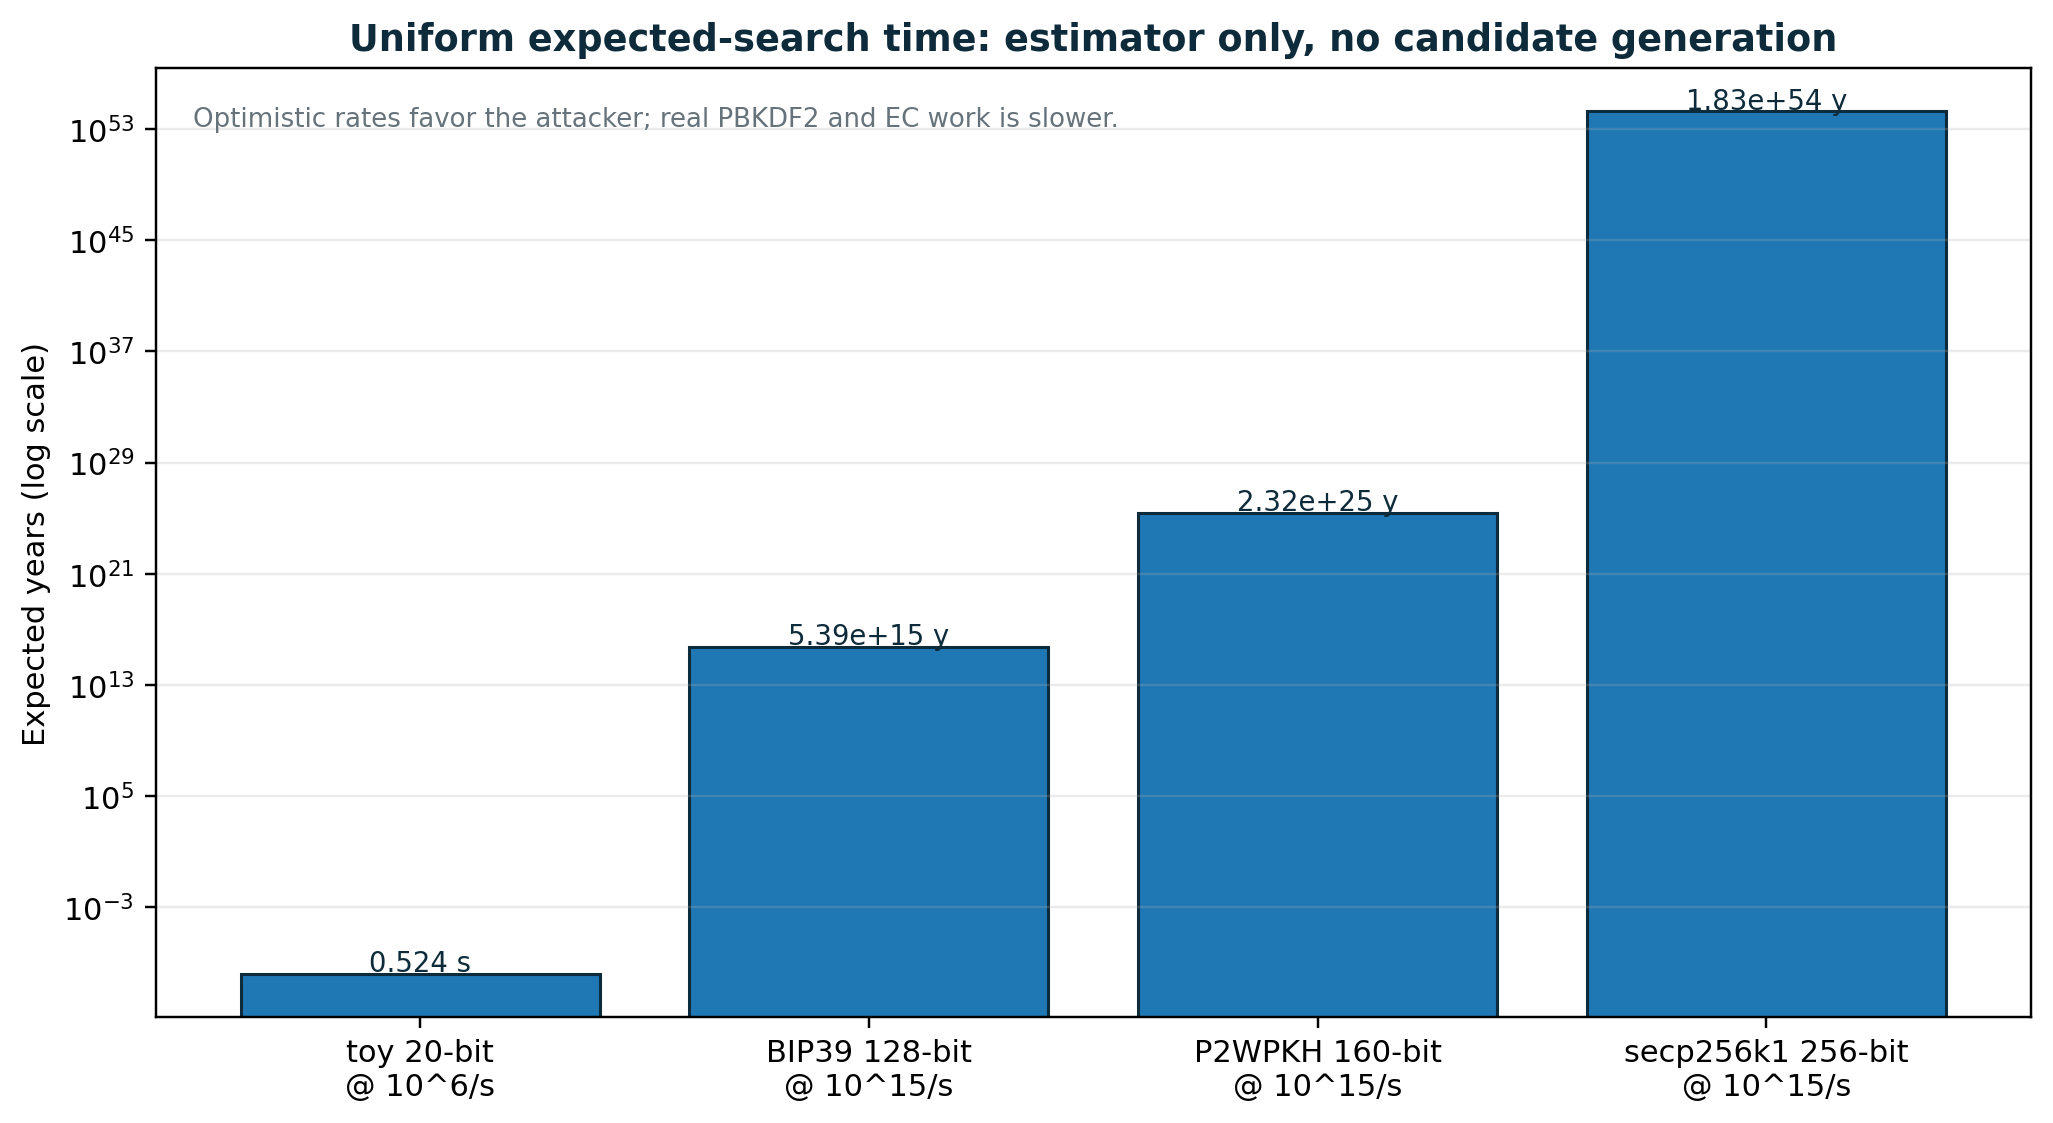
\includegraphics[width=0.84\textwidth]{figures/sara363_search_metrics.png}
\caption{The logarithmic chart shows the expected-time gap between a toy space and cryptographic spaces. The package contains the estimator only.}
\end{figure}

\begin{proofbox}
For twelve words, the raw index sequence has $132$ bits. The checksum fixes four of them as a function of the other $128$, so exactly $2^{128}$ valid encodings remain. Checksum filtering reduces arbitrary 12-word sequences by a factor of 16; it does not turn the valid space into a tractable search.
\end{proofbox}

\begin{boundbox}
The displayed rates ignore PBKDF2 cost, elliptic-curve work, memory, I/O and coordination and therefore favor the hypothetical searcher. They are feasibility lower bounds, not performance claims. The reference implementation has no candidate generator. Any appearance of a real-wallet target immediately fails the authorization policy.
\end{boundbox}

\section{Canonical UGTS event handoff}

SARA certification is upstream of the established event sequence:
\[
\text{certificate}\to\text{support}\to\text{compatibility}\to\text{guard}
\to\text{verified event}\to\text{transition}\to\text{lineage}.
\]

\begin{figure}[H]
\centering
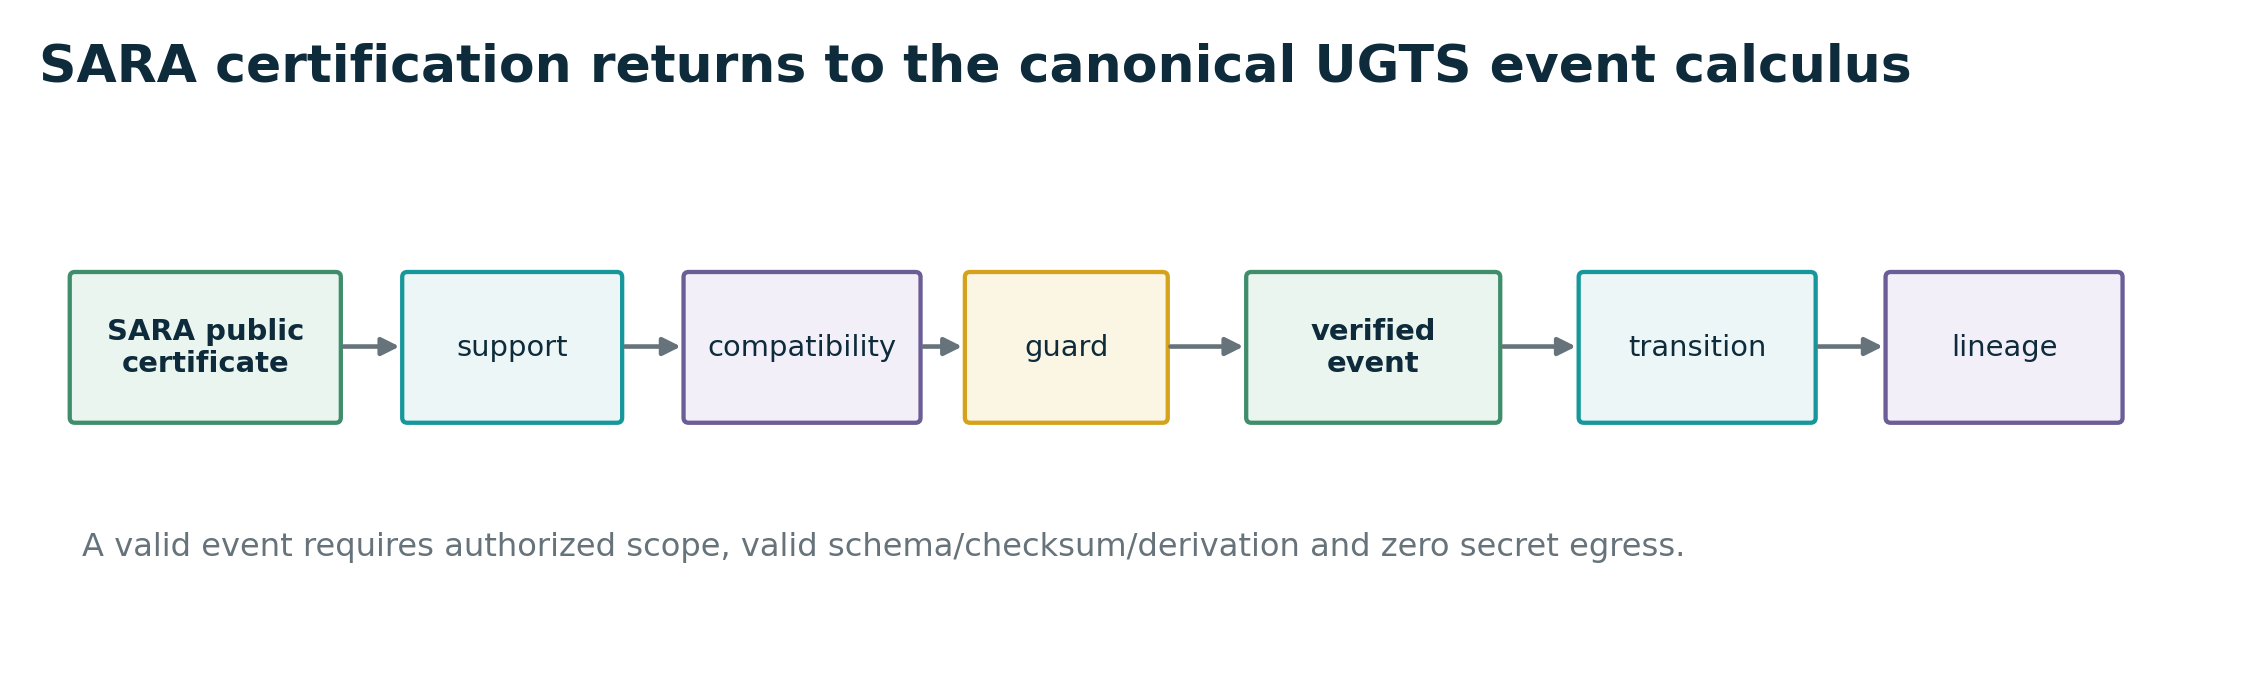
\includegraphics[width=0.92\textwidth]{figures/sara363_ugts_handoff.png}
\caption{Cryptographic certification does not replace the UGTS event calculus; it supplies a typed public relation and authorization result.}
\end{figure}

A practical mapping is:
\begin{center}
\begin{tabularx}{0.96\textwidth}{p{0.18\textwidth}X}
\toprule
\textbf{UGTS stage} & \textbf{SARA meaning}\\
\midrule
Support & Requested audit scope is local, declared and authorized.\\
Compatibility & Network, address family, derivation profile, schema and wordlist commitment agree.\\
Guard & Checksum, public vector, round-trip, secret-egress and capability predicates pass.\\
Verified event & A public-only certificate is issued with reason codes and residual/status fields.\\
Transition & Public state or watch-only metadata may be updated; secret state is never appended.\\
Lineage & Profile version, definition hashes, public inputs, test-vector IDs and audit decisions are recorded.\\
\bottomrule
\end{tabularx}
\end{center}

\section{Reference implementation}

\subsection{Modules}
\begin{center}
\small
\begin{tabularx}{0.97\textwidth}{>{\RaggedRight\arraybackslash}p{0.40\textwidth}X}
\toprule
\textbf{Path} & \textbf{Responsibility}\\
\midrule
\nolinkurl{src/ugts36/sara363.py} & BIP39 validation, BIP32/BIP84 public test derivation, Bech32/Bech32m codecs, public address decode, authorization and metrics.\\
\nolinkurl{src/ugts36/sara_runtime.py} & Six-step traceable, non-networked public certificate runtime.\\
\nolinkurl{spec/SARA_3_6_3_FORMAL_DEFINITION.md} & Concise normative definition.\\
\nolinkurl{spec/ugts_kc_3_6_3_sara.schema.json} & JSON Schema for the literal substrate.\\
\nolinkurl{examples/ugts_kc_3_6_3_sara_example.json} & Nineteen content-addressed definitions and pipeline references.\\
\nolinkurl{data/bip39_english.txt} & Official ordered 2048-word public list fixture.\\
\nolinkurl{data/sara363_public_address_fixture.json} & Public decode result for the supplied address.\\
\nolinkurl{data/sara363_search_space_metrics.*} & Estimator outputs; no candidate material.\\
\nolinkurl{tests/test_sara363.py} & Forty-two SARA tests.\\
\bottomrule
\end{tabularx}
\end{center}

\subsection{Bounded API}
The public reference functions include wordlist commitment, entropy-to-mnemonic conversion for known entropy, mnemonic checksum validation, known-input seed transition, BIP84 public certificate derivation, Bech32/Bech32m encode/decode, public-address decode, authorization and work estimation. The runtime deliberately exposes no search, signing, PSBT, network, balance or broadcast API.

\begin{Verbatim}[breaklines=true,fontsize=\small]
PYTHONPATH=src python examples/demo_sara363.py
PYTHONPATH=src python -m unittest discover -s tests -v
\end{Verbatim}

\subsection{Implementation boundary}
The elliptic-curve code is a dependency-free oracle for test vectors, not a production wallet library. Production systems require hardened, reviewed cryptographic libraries, secure entropy, side-channel protection, zeroization, isolated signing and audited custody. Passing this report's tests establishes internal conformance only.

\section{Validation and exact package metrics}

\begin{metricbox}
\begin{tabularx}{0.96\textwidth}{X r}
SARA 3.6.3 tests & 42 passed\\
Retained 3.6/3.6.1/3.6.2 tests & 153 passed\\
Combined tests & 195 passed\\
SARA operator records & 45\\
Content-addressed definitions & 19\\
Claims-ledger entries & 20\\
JSON Schema validation errors & 0\\
Invalid definition hashes & 0\\
Reference dependency cycles & 0\\
Official BIP84 public vector matches & 3\\
Supplied-address Bech32 round-trip & pass\\
Public certificate secret fields & 0\\
Runtime network capability & false\\
Runtime transaction capability & false\\
Reference certificate valid & true\\
\end{tabularx}
\end{metricbox}

The full test suite covers wordlist count and digest, entropy/checksum segmentation, known BIP39 seed output, BIP32 path parsing and child derivation, three BIP84 public vectors, Bech32 and Bech32m vectors, mixed-case and checksum rejection, witness-program length rules, authorization rejection, estimator bounds, secret-free serialization, JSON Schema, content hashes, dependency order and requester attribution.

\section{Claims ledger and kill criteria}

\subsection{Kill criteria}
The profile is stopped or simplified when any of the following occurs:
\begin{itemize}
\item scope cannot be proven public, self-owned or test-network authorized;
\item a secret appears in a serialized definition, trace, log or certificate;
\item a new function adds candidate enumeration, target comparison, signing, broadcast or funds transfer;
\item a checksum result is presented as ownership or authentication;
\item a public address label is presented as legal proof;
\item a production claim relies only on dependency-free oracle code or public vectors;
\item path, network, witness version, checksum family or program length is implicit rather than typed;
\item performance rhetoric is substituted for measured error, rate and authorization boundaries.
\end{itemize}

\subsection{Complete SARA claims ledger}
\begin{landscape}
\small
\setlength{\tabcolsep}{3pt}\begin{longtable}{@{}p{0.09\linewidth} p{0.33\linewidth} p{0.09\linewidth} p{0.40\linewidth}@{}}
\toprule
\textbf{ID} & \textbf{Claim} & \textbf{Disposition} & \textbf{Technical note}\\
\midrule
\endfirsthead
\toprule
\textbf{ID} & \textbf{Claim} & \textbf{Disposition} & \textbf{Technical note}\\
\midrule
\endhead
SARA-C001 & A BIP39 mnemonic is a human-created sentence or brainwallet. & REJECT & BIP39 transports computer-generated entropy and explicitly warns against user-created sentences.\\
\addlinespace[1.5pt]
SARA-C002 & The checksum adds independent secret entropy. & CORRECT & The checksum constrains valid encodings and catches some errors; valid mnemonic count remains 2\textasciicircum{}ENT.\\
\addlinespace[1.5pt]
SARA-C003 & A valid mnemonic checksum proves the owner or wallet balance. & REJECT & Checksum validity is syntax/integrity only.\\
\addlinespace[1.5pt]
SARA-C004 & The PBKDF2 step makes weak user passphrases unguessable. & BOUND & BIP39 fixes 2048 iterations; passphrase quality remains security-critical.\\
\addlinespace[1.5pt]
SARA-C005 & A public Bitcoin address can be inverted to its private key. & REJECT & The address exposes a script commitment and checksum, not spend authority.\\
\addlinespace[1.5pt]
SARA-C006 & Any hash collision can spend a specific P2WPKH output. & REJECT & A target preimage matching the witness program and a valid signature path are required; generic collision rhetoric is not sufficient.\\
\addlinespace[1.5pt]
SARA-C007 & A Bech32 checksum authenticates the wallet owner. & REJECT & It detects transcription errors; it is not authentication.\\
\addlinespace[1.5pt]
SARA-C008 & An address label on a block explorer proves legal ownership. & REJECT & Labels are external metadata and require independent provenance.\\
\addlinespace[1.5pt]
SARA-C009 & A 32-bit BIP32 parent fingerprint is a collision-free identity. & REJECT & It is a short identifier and implementations must tolerate collisions.\\
\addlinespace[1.5pt]
SARA-C010 & An extended public key is harmless public information. & BOUND & It cannot sign by itself but can reveal address families, balances and privacy-sensitive structure.\\
\addlinespace[1.5pt]
SARA-C011 & Hardened and normal derivation edges are interchangeable. & REJECT & Hardened children cannot be derived from an extended public parent.\\
\addlinespace[1.5pt]
SARA-C012 & A Bitcoin address is the same object as a key or wallet. & REJECT & Address, script, public key, extended node, seed and mnemonic are distinct typed objects.\\
\addlinespace[1.5pt]
SARA-C013 & The supplied public address authorizes private-key testing because it is public. & REJECT & Public visibility does not confer authorization to access or spend funds.\\
\addlinespace[1.5pt]
SARA-C014 & Brute force against a uniformly random 12-word mnemonic is a practical test plan. & REJECT & The valid keyspace is 2\textasciicircum{}128 and the reference metric is astronomically large even at unrealistic rates.\\
\addlinespace[1.5pt]
SARA-C015 & Address-targeted key search belongs in the reference package. & REJECT & The package provides decoding and feasibility metrics only, not search or candidate generation.\\
\addlinespace[1.5pt]
SARA-C016 & Mainnet and test networks are equivalent audit environments. & REJECT & Training and destructive experiments belong on regtest, signet, testnet or self-owned fixtures.\\
\addlinespace[1.5pt]
SARA-C017 & Seed or mnemonic may be stored in the UGTS lineage log. & REJECT & Secrets are transient and prohibited from definitions, traces and certificates.\\
\addlinespace[1.5pt]
SARA-C018 & The same mnemonic words translated into another language preserve the seed. & REJECT & BIP39 seed derivation hashes the normalized sentence; translation changes the seed.\\
\addlinespace[1.5pt]
SARA-C019 & One bit can represent the full wallet state. & REJECT & Checksums, keys, paths, scripts, policy, uncertainty and lineage remain separate.\\
\addlinespace[1.5pt]
SARA-C020 & Passing public test vectors proves production wallet security. & REJECT & It establishes reference conformance only; production security needs hardened libraries, secure entropy and key custody.\\
\addlinespace[1.5pt]
\bottomrule
\end{longtable}
\end{landscape}

\section{Final formal definition}

\begin{decisionbox}
UGTS-KC 3.6.3 SARA is a content-addressed, typed, public-certificate layer over deterministic-wallet standards. It maps BIP39 words into an ordered one-dimensional cell complex; validates the checksum as a guard; treats the seed and private HD nodes as transient; represents BIP32 derivation as a labeled tree with distinct normal and hardened edges; projects only to public keys, witness programs, scripts and addresses; decodes the supplied address as a public fixture; evaluates search-space size without enumeration; rejects unauthorized secret/funds-access scopes; and hands a valid public certificate to the canonical UGTS support--compatibility--guard--event--transition--lineage sequence.
\end{decisionbox}

The title ``SARA'' is an engineering-derived abbreviation for \emph{Seed-Address Referential Algebra}. It is not a Bitcoin standard name and does not imply endorsement by Bitcoin contributors, a wallet provider or a public authority.

\section{Complete SARA 3.6.3 operator catalog}
\begin{landscape}
\scriptsize
\setlength{\tabcolsep}{3pt}\begin{longtable}{@{}p{0.17\linewidth} p{0.09\linewidth} p{0.15\linewidth} p{0.32\linewidth} p{0.10\linewidth} p{0.08\linewidth}@{}}
\toprule
\textbf{ID} & \textbf{Domain} & \textbf{Name} & \textbf{Formal definition} & \textbf{Disposition} & \textbf{Validation}\\
\midrule
\endfirsthead
\toprule
\textbf{ID} & \textbf{Domain} & \textbf{Name} & \textbf{Formal definition} & \textbf{Disposition} & \textbf{Validation}\\
\midrule
\endhead
sara363.profile.v1 & Profile & Seed-address referential algebra & Typed BIP39/BIP32/BIP84/Bech32 profile with public-only certificates and an authorization gate. & ENGINEERING-DERIVED & Implemented\\
\addlinespace[1.5pt]
sara363.governance.evidence-boundary & Governance & Source and standards boundary & Separate BIP-defined transformations, engineering glue, public fixtures, metrics and rejected attack scopes. & RETAIN & Enforced\\
\addlinespace[1.5pt]
sara363.security.secret-class & Security & Secret/public classification & Entropy, mnemonic, passphrase, seed, private scalar and chain code are secret; addresses, scripts and test vectors are public. & ENGINEERING-DERIVED & Implemented\\
\addlinespace[1.5pt]
sara363.wordlist.commitment & Encoding & 2048-word list commitment & Bind the selected BIP39 wordlist by count, order, uniqueness, normalization and SHA-256 digest. & RETAIN & Exact\\
\addlinespace[1.5pt]
sara363.entropy.input & Encoding & Computer-generated entropy input & Admit only ENT in \{128,160,192,224,256\}; do not treat arbitrary user sentences as entropy. & RETAIN & Exact\\
\addlinespace[1.5pt]
sara363.checksum.prefix & Encoding & BIP39 checksum prefix & CS=ENT/32 and checksum bits are the first CS bits of SHA-256(entropy). & RETAIN & Exact\\
\addlinespace[1.5pt]
sara363.bits.concat & Encoding & Entropy-checksum concatenation & Append checksum bits to entropy before word segmentation. & RETAIN & Exact\\
\addlinespace[1.5pt]
sara363.bits.segment11 & Encoding & Eleven-bit segmentation & Split ENT+CS into ordered 11-bit cells, each in [0,2047]. & RETAIN & Exact\\
\addlinespace[1.5pt]
sara363.words.lookup & Encoding & Word-index lookup & Map each 11-bit cell to one word in the committed list. & RETAIN & Exact\\
\addlinespace[1.5pt]
sara363.words.cell-complex & Topology & Ordered word-cell complex & Represent the mnemonic as a 1D path of labeled 11-bit cells whose adjacency preserves word order. & TRANSLATE & Specified\\
\addlinespace[1.5pt]
sara363.mnemonic.checksum-hinge & Event calculus & Mnemonic checksum hinge & A mnemonic is admitted only when observed checksum cells equal the entropy-hash prefix. & TRANSLATE & Implemented\\
\addlinespace[1.5pt]
sara363.text.nfkd & Encoding & Unicode NFKD normalization & Normalize mnemonic and passphrase as required before seed derivation. & RETAIN & Implemented\\
\addlinespace[1.5pt]
sara363.seed.pbkdf2 & Cryptography & Mnemonic-to-seed transition & PBKDF2-HMAC-SHA512 with 2048 iterations, 64-byte output and salt 'mnemonic'+passphrase. & RETAIN & Implemented\\
\addlinespace[1.5pt]
sara363.seed.no-serialization & Security & Seed nonserialization & Seed bytes are transient and excluded from substrate definitions, traces, certificates and package data. & ENGINEERING-DERIVED & Enforced\\
\addlinespace[1.5pt]
sara363.bip32.master & Cryptography & BIP32 master node & HMAC-SHA512 with key 'Bitcoin seed' creates a private scalar and 32-byte chain code. & RETAIN & Implemented\\
\addlinespace[1.5pt]
sara363.bip32.node & Topology & Extended-key tree node & Node state is key material plus chain code, depth, parent fingerprint and child number. & RETAIN & Implemented\\
\addlinespace[1.5pt]
sara363.bip32.normal-edge & Topology & Normal derivation edge & Indices below 2\textasciicircum{}31 admit private and public child derivation under BIP32 rules. & RETAIN & Private path implemented\\
\addlinespace[1.5pt]
sara363.bip32.hardened-edge & Topology & Hardened derivation edge & Indices at or above 2\textasciicircum{}31 require parent private material and block public-parent derivation. & RETAIN & Private path implemented\\
\addlinespace[1.5pt]
sara363.path.parser & Encoding & Derivation-path parser & Parse m/... with explicit hardened markers and uint32 bounds. & ENGINEERING-DERIVED & Implemented\\
\addlinespace[1.5pt]
sara363.path.bip44 & Information architecture & Five-level account hierarchy & Purpose/coin/account/change/index are distinct typed path levels. & RETAIN & Specified\\
\addlinespace[1.5pt]
sara363.path.bip84 & Information architecture & Native P2WPKH derivation policy & Use m/84'/coin'/account'/change/index for BIP84 accounts. & RETAIN & Implemented\\
\addlinespace[1.5pt]
sara363.ec.secp256k1 & Cryptography & secp256k1 public projection & Map a valid scalar to a curve point without exposing a signing API. & RETAIN & Reference implementation\\
\addlinespace[1.5pt]
sara363.pubkey.compressed & Encoding & Compressed public key & Serialize a curve point as parity prefix plus 32-byte x coordinate. & RETAIN & Implemented\\
\addlinespace[1.5pt]
sara363.hash.hash160 & Cryptography & HASH160 commitment & RIPEMD160(SHA256(compressed public key)) yields the 20-byte P2WPKH witness program. & RETAIN & Implemented\\
\addlinespace[1.5pt]
sara363.script.p2wpkh & Relation & P2WPKH script relation & Witness v0 with a 20-byte key hash maps to scriptPubKey 0x0014\{program\}. & RETAIN & Implemented\\
\addlinespace[1.5pt]
sara363.address.convertbits & Encoding & Eight-to-five-bit regrouping & Convert witness-program bytes into 5-bit Bech32 data groups with canonical padding. & RETAIN & Implemented\\
\addlinespace[1.5pt]
sara363.address.hrp & Encoding & Human-readable prefix & Bind the network namespace through HRP such as bc or tb. & RETAIN & Implemented\\
\addlinespace[1.5pt]
sara363.address.bech32 & Encoding & Bech32 checksum shell & Witness version 0 addresses use the BIP173 polymod constant. & RETAIN & Implemented\\
\addlinespace[1.5pt]
sara363.address.bech32m & Encoding & Bech32m checksum shell & Witness versions 1-16 use the BIP350 polymod constant. & RETAIN & Implemented\\
\addlinespace[1.5pt]
sara363.address.decode & Query & Public address decoder & Validate case, HRP, checksum family, witness version, program length and script projection. & ENGINEERING-DERIVED & Implemented\\
\addlinespace[1.5pt]
sara363.address.classify & Query & Witness-program classifier & Classify v0/20 as P2WPKH, v0/32 as P2WSH and v1/32 as a Taproot-compatible form. & ENGINEERING-DERIVED & Implemented\\
\addlinespace[1.5pt]
sara363.address.noninverse & Security & Non-reversibility boundary & Address decoding exposes a script commitment, not a private key, seed or spend authority. & CORRECTED & Enforced\\
\addlinespace[1.5pt]
sara363.fixture.public-address & Fixture & User-supplied public address fixture & Use the supplied bc1q address only for format, checksum, witness-program and scriptPubKey validation. & BOUNDED & Verified\\
\addlinespace[1.5pt]
sara363.audit.self-owned & Audit & Self-owned known-seed audit & Permit deterministic backup verification only when the operator already possesses the mnemonic or seed. & BOUNDED & Policy\\
\addlinespace[1.5pt]
sara363.audit.watch-only & Audit & Watch-only public audit & Permit address/descriptor parsing and public derivation evidence without spend authority. & BOUNDED & Policy\\
\addlinespace[1.5pt]
sara363.audit.authorization-gate & Governance & Authorization gate & Every audit declares a scope and is rejected if any operation targets private keys, third-party secrets or funds. & ENGINEERING-DERIVED & Implemented\\
\addlinespace[1.5pt]
sara363.audit.forbidden-search & Governance & Forbidden-target rejection & Reject mnemonic enumeration, passphrase spraying, private-key scanning and address-targeted preimage search. & REJECT & Enforced\\
\addlinespace[1.5pt]
sara363.audit.no-network & Security & No-network reference runtime & The reference implementation performs no blockchain queries, balance lookups or remote calls. & ENGINEERING-DERIVED & Enforced\\
\addlinespace[1.5pt]
sara363.audit.no-signing & Security & No-signing reference runtime & The reference implementation exposes no transaction signing, PSBT mutation, broadcast or funds-transfer path. & ENGINEERING-DERIVED & Enforced\\
\addlinespace[1.5pt]
sara363.metric.uniform-search & Metric & Uniform search-space estimator & Report 2\textasciicircum{}b candidates, 2\textasciicircum{}(b-1) expected guesses and time at a declared optimistic rate; do not enumerate. & ENGINEERING-DERIVED & Implemented\\
\addlinespace[1.5pt]
sara363.metric.bip39-valid-space & Metric & Valid mnemonic keyspace & A 12-word BIP39 space contains 2\textasciicircum{}128 valid mnemonics; checksum filtering does not reduce the encoded entropy below ENT. & CORRECTED & Exact\\
\addlinespace[1.5pt]
sara363.metric.toy-space & Metric & Reduced synthetic metric & Use a 20-bit toy space only to explain scale; it is explicitly not a Bitcoin wallet or key search. & BOUNDED & Measured\\
\addlinespace[1.5pt]
sara363.certificate.public-only & Certificate & Public-only derivation certificate & Return path, parent routing fingerprint, compressed public key, HASH160, script and address while excluding mnemonic-, seed- and private-key-derived commitments. & ENGINEERING-DERIVED & Implemented\\
\addlinespace[1.5pt]
sara363.lineage.audit-record & Persistence & Audit lineage record & Log standards profile, public fixture digest, reason codes and test-vector result, never mnemonic/seed/private keys. & ENGINEERING-DERIVED & Specified\\
\addlinespace[1.5pt]
sara363.handoff.ugts & Architecture & Canonical UGTS handoff & After cryptographic certification, return to support, compatibility, guard, event, transition and lineage. & RETAIN & Specified\\
\addlinespace[1.5pt]
\bottomrule
\end{longtable}
\end{landscape}

\section{Package layout and reproduction}

\begin{Verbatim}[breaklines=true,fontsize=\small]
README.md / NOTICE.md / CHANGELOG.md / VERSION
report/      PDF, editable TeX, figures, preflight reports
spec/        formal definition, 45 operators, 20 claims, JSON Schema
src/ugts36/  SARA runtime plus retained 3.6/3.6.1/3.6.2 modules
tests/       195-test combined suite
examples/    literal substrate, public certificate and trace
data/        BIP39 wordlist, public address fixture, metrics
sources/     standards register and privacy-safe distillation notes
checksums/   SHA-256 manifest and package verification
\end{Verbatim}

No raw private wallet material, raw uploaded source PDFs, font files, network credentials or transaction artifacts are included.

\section*{Normative references}
\begin{itemize}
\item BIP 39, \emph{Mnemonic code for generating deterministic keys}: \url{https://github.com/bitcoin/bips/blob/master/bip-0039.mediawiki}
\item BIP 32, \emph{Hierarchical Deterministic Wallets}: \url{https://github.com/bitcoin/bips/blob/master/bip-0032.mediawiki}
\item BIP 44, \emph{Multi-account hierarchy}: \url{https://github.com/bitcoin/bips/blob/master/bip-0044.mediawiki}
\item BIP 84, \emph{Derivation scheme for P2WPKH accounts}: \url{https://github.com/bitcoin/bips/blob/master/bip-0084.mediawiki}
\item BIP 141, \emph{Segregated Witness}: \url{https://github.com/bitcoin/bips/blob/master/bip-0141.mediawiki}
\item BIP 173, \emph{Base32 address format for native witness outputs}: \url{https://github.com/bitcoin/bips/blob/master/bip-0173.mediawiki}
\item BIP 350, \emph{Bech32m format for v1+ witness addresses}: \url{https://github.com/bitcoin/bips/blob/master/bip-0350.mediawiki}
\item UGTS-KC 3.6.2 SCLP, inherited referential geometry/topology, packed state and canonical event handoff.
\end{itemize}

\end{document}
